\documentclass[border=0mm]{standalone}
\usepackage[T1]{fontenc}
\usepackage[utf8]{inputenc}
\usepackage[charter]{mathdesign}
\usepackage{tikz}

\begin{document}

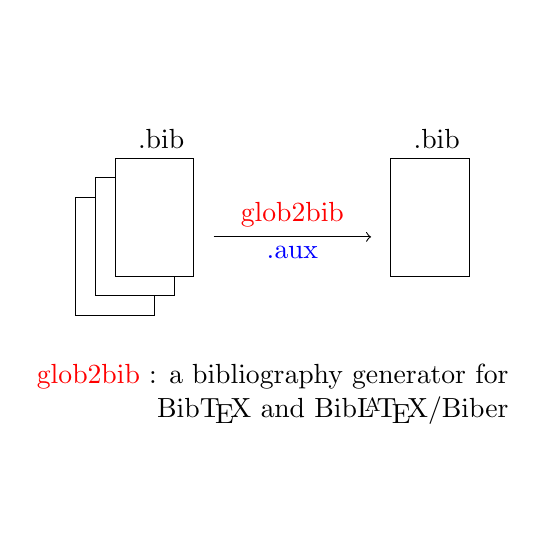
\begin{tikzpicture}

% command drawing dimensions
\newcommand{\offset}{0.25}
\newcommand{\rwidth}{1.0}
\newcommand{\rheight}{1.5}

\newcommand{\xorigin}{-0.60}
\newcommand{\yorigin}{-2.6}
\newcommand{\sdim}{6.25}

% ad hoc bounding box 
\draw[white] (\xorigin, \yorigin) rectangle (\xorigin + \sdim, \yorigin + \sdim);

% stack of rectangles
\draw[fill=white] (0, 0) rectangle (\rwidth, \rheight);
\draw[fill=white] (\offset, \offset) rectangle (\rwidth + \offset, \rheight + \offset);
\draw[fill=white] (2 * \offset, 2 * \offset) rectangle (\rwidth + 2 * \offset, \rheight + 2 * \offset) node[anchor=south east, align=center] {.bib};

% arrow 
\draw[->] (\rwidth + 3 * \offset, 0.5 * \rheight + \offset) -- (2 * \rwidth + 7 * \offset,  0.5 * \rheight + \offset) node[above, midway, align=center, red] {glob2bib} node[below, midway, align=center, blue] {.aux};

% rectangle
\draw[fill=white] (2 * \rwidth + 8 * \offset, 2 * \offset) rectangle (3 * \rwidth + 8 * \offset, \rheight + 2 * \offset) node[anchor=south east, align=center] {.bib};

%
\node[below, align=right] at (2 * \rwidth + 2 * \offset, -2 * \offset) {\textcolor{red}{glob2bib} : a bibliography generator for \\ Bib\TeX\ and Bib\LaTeX/Biber};

\end{tikzpicture}

\end{document}
